% !TEX root = ../main.tex
\newpage
\chapter{Архітектура та інформаційне забезпечення БД}
\section{Аналіз функціонування та організаційні засади підприємства}
До основних функціональних завдань ЗВО належить планування занять та формування їх розкладу,
облік викладачів та студентів, контроль успішності студентів.
Для зберігання необхідних даних доцільно сформувати такі таблиці:
<<Факультети>>, <<Кафедри>>, <<Групи>>, <<Студенти>>, <<Викладачі>>, 
<<Дисципліни>>, <<Розклад>> та <<Сесія>>. На кожному факультеті є кафедри,
за якими закріплені викладачі та навчальні групи студентів. В таблиці <<Дисципліни>>
має бути загальний перелік дисциплін, а вже в таблиці <<Розклад>> -- розподіл
дисциплін за групами та викладачами.

\section{Проектування структури бази даних}
Структуру таблиць БД та зв'язки між ними зображено на EER-діаграмі:
\begin{figure}[h]
    \centering
    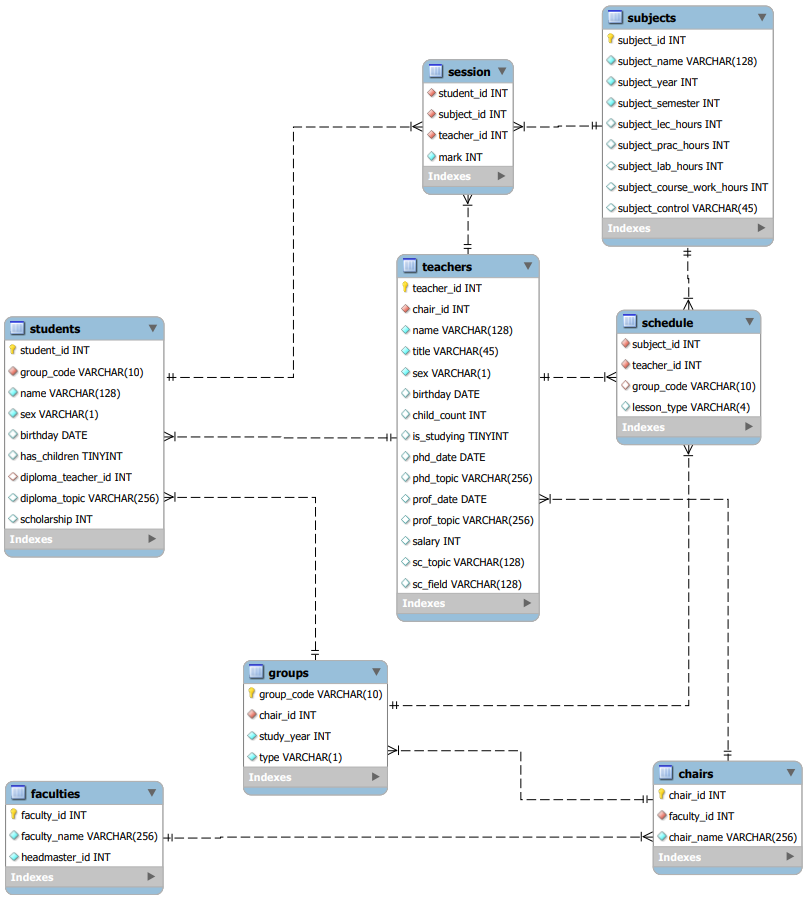
\includegraphics[scale=0.8]{pics/eer.png}
    \caption{EER-діаграма}
\end{figure}

Зв'язки між різними таблицями реалізовано через механізм Foreign Key.
Наприклад, в таблиці <<Сесія>> поля subject\_id, student\_id, teacher\_id 
пов'язані з однойменними полями, що є Primary Key, в таблицях <<Дисципліни>>, <<Студенти>> та <<Викладачі>>.

\section{Життєві цикли бази даних}
\begin{enumerate}
    \item Попереднє планування. На даному етапі було сформовано модель структури бази даних, визначено сутності та
    проаналізовано зв'язки між ними.
    \item Перевірка здійсненності. Для розробки даної системи необхідно мати встановлений сервер MySQL 8.0,
    інтерпретатор мови Python 3.9 з найновішими версіями фреймворку Flask і бібліотеки PyMySQL та
    середовище розробки MySQL Workbench. 
\end{enumerate}